\documentclass[a4paper,11pt]{article}
\usepackage[top = 1.5 in, bottom = 1 in, left = 1.5 in, right = 1.5 in]{geometry}
\usepackage[utf8]{inputenc}
\usepackage[T1]{fontenc}
\usepackage[british, finnish]{babel}
\usepackage{lmodern}
\usepackage{url}
\usepackage{color}
\usepackage{graphicx}
\usepackage{setspace}
\usepackage{biblatex}
\bibliography{lahteet}
\newcommand{\engl}[1]{\foreignlanguage{english}{\em #1}}

\begin{document}
\title{Järjestämisalgoritmien suunnittelu grafiikkayksiköille}
\author{Laura Leppänen}
\date{\today}
\maketitle
\thispagestyle{empty}

\tableofcontents
\onehalfspacing

\newpage
\setcounter{page}{1}

\section{Johdanto}

Järjestäminen on yksi tunnetuimmista ja tutkituimmista laskennallisista ongelmista. Järjestämisalgoritmit ovat keskeisiä rakennuspalikoita esimerkiksi tietokantajärjestelmissä, hakumoottoreissa sekä tietokonegrafiikassa ja maantieteellistä dataa käsittelevissä järjestelmissä, joissa kohteita järjestetetään spatiaalisesti. Tästä johtuen tehokkaita järjestämisalgoritmeja tarvitaan kaikilla ohjelmointialustoilla, ja uusien arkkitehtuurien tarjoamia rinnakkaistamismahdollisuuksia on tarpeen käyttää hyödyksi.

Prosessorien ytimien määrä on jo pitkään ollut jatkuvassa kasvussa. Neliytimiset suorittimet ovat jo nykyään tavallisia, ja tulevaisuudessa kehitys näyttää menevän yhä vahvemmin ns. massiivimoniytimisten prosessorien (\engl{manycore processor}) suuntaan. Lisäksi ytimet kykenevät usein useamman säikeen suorittamiseen yhtäaikaisesti. Grafiikkayksiköissä massiivinen ytimien määrä on jo saavutettu: esimerkiksi nykyisissä Nvidian valmistamissa grafiikkayksiköissä ytimiä on jopa 448 kappaletta (Nvidia Tesla C2050/ C2070/C2075) \cite{nvidiafermi2010}.

Ytimien määrän lisäksi grafiikkayksiköiden ohjelmoinnissa täytyy ottaa huomioon, että ulkoiseen muistiin viittaaminen on hidasta, ja grafiikkapiirillä olevaa nopeaa muistia on rajallinen määrä \cite{leischner2010}. Täten muistissakäynnit on syytä suunnitella siten, että grafiikkayksikkö pystyy yhdistämään joukon muistiviittauksia yhdeksi viittaukseksi suurempaan muistialueeseen.

Esittelen seuraavassa luvussa lyhyesti CUDA-ohjelmointiympäristön ja ne grafiikkayksiköiden arkkitehtuuriset ominaisuudet, jotka algoritmien suunnittelussa on otettava huomioon. Sen jälkeen esittelen muutamia erityyppisiä järjestämisalgoritmeja ja niiden toteutuksia CUDA-ympäristössä.

\section{Rinnakkaislaskenta nykyisillä grafiikkayksiköillä}

\subsection{Tesla-näytönohjaimet ja CUDA-arkkitehtuuri}

Edellisen sukupolven Tesla-näytönohjaimissa (C1060) oli 30 moniprosessoria \\ (\engl{streaming multiprocessor}), joista jokainen koostuu kahdeksasta ytimestä (\engl{scalar processor}). Yhteensä fyysisiä ytimiä oli siis 240. Uusimman sukupolven Tes\-la-näy\-tön\-oh\-jai\-mis\-sa ytimiä on 448 jaettuna 14 moniprosessorille. Tesla-gra\-fiik\-ka\-yk\-si\-kön täydellinen hyödyntäminen kuitenkin edellyttää vähintään n. 5000\thinspace--\thinspace10\thinspace000 yhtäaikaisen säikeen käyttöä \cite{leischner2010}. Yksittäisellä Tesla C1060 -näytönohjaimen moniprosessorilla on mahdollista ajaa yhtäaikaisesti 1024 säiettä \cite{satish2009}.

Jokaisella moniprosessorilla on tietty näytönohjaimen sukupolvesta riippuva määrä rekisteritilaa. Lisäksi jokaisella moniprosessorilla on oma ydinten kesken jaettu muisti, jonka luku- ja kirjoitusoperaatiot ovat nopeita. Viittaukset ulkoiseen muistiin pyritään minimoimaan, koska ne ovat kalliita operaatioita.

Hallitakseen suurta määrää yhtäaikaisia säikeitä moniprosessorit käyttävät ns. SIMT-arkkitehtuuria (\engl{Single Instruction, Multiple Thread}) \cite{lindholm2008}. Moniprosessorin SIMT-käsky-yksikkö suorittaa säikeet 32 rinnakkaisen säikeen ryhmissä eli ns. loimissa (\engl{warp}, Lindholmin \cite{lindholm2008} mukaan termi on peräisin matonkudonnasta). Loimen säikeet ovat kaikki samaa tyyppiä, mutta käyttävät eri dataa.

CUDA-ohjelmointiympäristö (\engl{Compute Unified Device Architecture}) \cite{cudaprogramming} mahdollistaa rinnakkaisten ohjelmien ajamisen näytönohjaimilla. Tyypillisesti (sarjalliset) CUDA-isäntäsovellukset suoritetaan tavallisella suorittimella ja rinnakkaiset aliohjelmat (CUDA-ytimet, \engl{kernels}) näytönohjaimella.

CUDA-ytimet ovat sarjallisia sovelluksia, joita suoritetaan useassa säikeessä samanaikaisesti. Nämä säikeet järjestetään säielohkoiksi (\engl{thread block}) \cite{cudaprogramming}. Analysoitaessa CUDA-ohjelmointiympäristölle suunniteltuja algoritmeja voidaan ajatella käytettävien säielohkojen määrän vastaavan prosessorien määrää perinteisemmässä rinnakkaisalgoritmien analyysissa \cite{satish2009}.

\subsection{Suorituskyvyn tehostaminen}

Jotta näytönohjainten täyttä tehoa pystyttäisiin hyödyntämään, täytyy algoritmien suunnittelussa huomioida joitakin SIMT-arkkitehtuureihin liittyviä erityisominaisuuksia.

Loimeen kuuluvat säikeet suoritetaan siten, että jokainen säie suorittaa samaa käskyä samanaikaisesti, mutta kukin niistä käsittelee eri dataa (ns. SIMD-käskyt, \engl{Single Instruction, Multiple Data}). Jos kaksi säiettä haarautuu eri suuntiin valintalauseessa, valitut haarat suoritetaan peräkkäin --- ei siis rinnakkain \cite{leischner2010} \cite{cederman2009}. Tämä hidastaa suoritusta, joten täysi teho saavutetaan vain, jos kaikki saman loimen säikeet valitsevat saman suorituspolun. Eri loimien välisillä eroilla sen sijaan ei ole merkitystä suorituskyvyn kannalta \cite{leischner2010} \cite{satish2009}.

Suorituksen aikana data pidetään globaalissa muistissa, mutta siihen viittaaminen on melko hidasta. Kullakin moniprosessorilla on näytönohjainmallista riippuva määrä nopeaa paikallista muistia --- esimerkiksi Tesla C1060-näytönohjaimella 16 kilotavua moniprosessoria kohti. Laskennan aikana kannattaa siis käyttää paikallista jaettua muistia datan väliaikaiseen säilytykseen, koska viittauksia muistiin tulee paljon \cite{cederman2009} \cite{leischner2010}. Laskennan loputtua käsitelty data voidaan kopioida takaisin globaaliin muistiin.

Säikeet voivat periaatteessa viitata mihin tahansa kohtaan muistia, mutta muistiviittaukset kannattaa tehdä siten, että samaan loimeen kuuluvat säikeet viittaavat peräkkäisiin muistiosoitteisiin. Tällöin muistiviitteet voidaan muuntaa yhdeksi suureksi luku- tai kirjoitusoperaatioksi \cite{cederman2009} \cite{satish2009}. Paikallista jaettua muistia käytettäessä säikeiden kannattaa viitata eri muistipaikkoihin, koska muutoin luku- ja kirjoitusoperaatiot joudutaan taas suorittamaan sarjallisesti. Toisaalta jos kaikki säikeet viittaavat samaan muistipaikkaan, tulee muistiviitteestä taas yhtä nopea kuin yksittäisestä lukuoperaatiosta \cite{cederman2009}.

\section{Järjestämisalgoritmit CUDA-ympäristölle}

Tehokkaimpia tähän mennessä julkaistuja järjestämisalgoritmeja CUDA-ym\-pä\-ris\-töl\-le näyttävät kirjallisuuden perusteella olevan eri toteutukset lomitusjärjestämisestä (\engl{merge sort}) \cite{satish2009} \cite{satish2010}, kantalukujärjestämisestä (\engl{radix sort}) \cite{satish2009} \cite{merrill2010} \cite{satish2010} ja laskentajärjestämisestä (\engl{counting sort}) \cite{kolonias2011}. Myös järjestämisverkkoihin perustuvat algoritmit kuten Petersin ja Schulz-Hildebrandtin \cite{peters2012gems} esittelemä toteutus bitoniselle järjestämisalgoritmille (\engl{bitonic sort}) näyttävät lupaavalta lähestymistavalta massiivimoniytimisillä prosessoreilla suoritettavaan järjestämiseen.

Myös pikajärjestämisestä (\engl{quicksort}), jota on perinteisesti pidetty yhtenä nopeimmista lajittelualgoritmeista yksiytimisillä prosessoreilla, on tehty joitakin toteutuksia CUDAlle (mm. \cite{cederman2009}), mutta toteutukset ovat olleet melko monimutkaisia, eivätkä ole siitä huolimatta aivan pärjänneet esimerkiksi yksinkertaiselle kantalukujärjestämiselle.

\subsection{Kantalukujärjestäminen}

Kantalukujärjestäminen on kokonaislukuavainten järjestämiseen tarkoitettu algoritmi, joka perustuu luvun numeroiden järjestämiseen yksitellen vähiten merkitsevästä numerosta\footnote{Huom: Jos siis kantaluku (\engl{radix}) on 10, tarkoitetaan tässä numerolla kokonaislukuja 0\thinspace--\thinspace9. Kantaluku voisi kuitenkin olla esimerkiksi 2, jolloin käsiteltäisiin kokonaislukujen sijaan avaimen bittiesityksen yksittäisiä bittejä.} alkaen. Kun kokonaislukuavainten pituus on vakio $d$ ja avaimia on $n$ kappaletta, algoritmin aikavaativuus on $O(n)$.

Algoritmi käy avaimet läpi $d$ kertaa. Jokaisella läpikäynnillä avainjoukko järjestetään yksittäisen avaimen numeron perusteella käyttäen jotakin vakaata\footnote{Järjestämisalgoritmi on \emph{vakaa}, jos se säilyttää sellaisten arvojen alkuperäisen järjestyksen, joiden avaimet ovat yhtä suuret. Esimerkiksi parijono $(3, 7)$, $(3, 1)$ voidaan järjestää parin ensimmäisen alkion perusteella kahdella eri tavalla. Vakaan järjestämisalgoritmin tulos olisi $(3, 7)$, $(3, 1)$. Epävakaa järjestämisalgoritmi voisi tuottaa tuloksen $(3, 1)$, $(3, 7)$.} järjestämisalgoritmia, esimerkiksi laskentajärjestämistä \cite{clrs}. Juuri laskentajärjestämisen käyttäminen primitiivinä tekee kantalukujärjestämisestä helposti rinnakkaistuvan, sillä laskentajärjestäminen voidaan esimerkiksi helposti redusoida rinnakkaiseksi prefiksisummaoperaatioksi\footnote{Lukujonon $x_0, x_1, x_2, ..., x_n$ prefiksisumma on lukujono $x_0, x_0 + x_1, x_0 + x_1 + x_2, ..., x_0 + ... + x_n$.} \cite{satish2009}.

Satishin ja kumppanien \cite{satish2009} varhaisemmassa lähestymistavassa kantaluku on $2^b$, missä $b$ valitaan kokeellisesti. Tällöin kokonaislukuavaimen numerot ovat $b$ bitin jonoja. Tarvittavien muistiviitteiden (\engl{scatter}-operaatioiden) määrä pyritään minimoimaan valitsemalla $b > 1$. Data jaetaan 256 säikeen säielohkoihin, joista kukin käsittelee 1024 alkiota --- siis 4 alkiota säiettä kohti. Säielohkoja luodaan siis $p = \lceil n/1024 \rceil$ kappaletta \cite{satish2009}.

Jokaista kokonaislukuavaimen $k$ numeroa kohti lasketaan monessako avaimessa esiintyy samassa kohtaa pienempi numero, ja kuinka monta sellaista avainta, joissa numero on sama, esiintyy aikaisemmin lukujonossa. Näiden kahden lukumäärän summa on avaimen $k$ indeksi eli aste (\engl{rank}) järjestämisen tuloksena saatavassa taulukossa \cite{satish2009}. Tehokkuuden vuoksi tämä tehdään siten, että jokainen säielohko laskee histogrammin sille annetun lukujoukon lukujen esiintymistä, jolloin asteet voidaan helposti laskea prefiksisumman avulla.

Läpikäynnit suoritetaan neljässä vaiheessa:
\singlespacing
\begin{enumerate}
\item Kukin säielohko järjestää sille kuuluvat alkiot paikallisessa nopeassa muistissa. Bitit käsitellään yksitellen siten, että iteraatioita tulee $b$ kappaletta.
\item Kukin säielohko kirjoittaa numeroiden esiintymähistogrammin ja järjestetyn datan globaaliin muistiin.
\item Lasketaan sarakkeittaisessa järjestyksessä (\engl{column-major order}) prefiksisumma $p$ kappaleesta histogrammitaulukoita. Ks. kuva \ref{fig:columnscan}.
\item Kukin säielohko kopioi alkionsa prefiksisummalla lasketun indeksin osoittamaan muistiosoitteeseen.
\end{enumerate}
\onehalfspacing

\begin{figure}
\centering
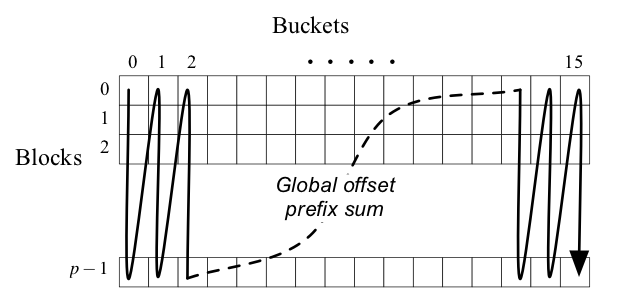
\includegraphics[scale = 0.5]{prefixsum}
\caption{Prefiksisumma sarakkeittaisessa järjestyksessä (kuvan lähde \cite{satish2009}). Taulukon rivit ovat eri säielohkojen tuottamia histogrammitaulukoita.}
\label{fig:columnscan}
\end{figure}

Kantaluvussa esiintyvän vakion $b$ valintaan vaikuttaa kaksi tekijää \cite{satish2009}. Toisaalta suuremmat $b$:n arvot heikentävät kohdassa (4) tapahtuvien \engl{scatter}-o\-pe\-raa\-ti\-oi\-den yhtenäisyyttä, koska mahdollisten numeroiden joukko on suurempi. Toisaalta jos $b$:n arvo on pienempi, joudutaan läpikäyntejä tekemään enemmän, jolloin jokaisen läpikäynnin lopussa suoritetaan uusi \engl{scatter}-operaatio muistiin. Molemmat ovat hidastavia tekijöitä. Kantaluvuksi $2^b$ valitaan empiirisen optimoinnin tuloksena $2^b = 16 = \sqrt{t}$, missä $b = 4$ ja $t = 256$ on säikeiden määrä yhdessä säielohkossa.

% Satish et al. 2009 & 2010
% Merrill & Grimshaw 2010

\subsection{Lomitusjärjestäminen}

% Satish et al. 2009 & 2010

\subsection{Laskentajärjestäminen}

% Kolonias et al.

%\subsection{Järjestämisverkot ja bitoninen järjestäminen}

% Käsitellään jos mahtuu
% Peters ja Hildebrandt

\printbibliography

\end{document}
